\documentclass{article}
\usepackage[utf8]{inputenc}
\usepackage{amssymb}
\usepackage{graphicx}
\usepackage{setspace}
\usepackage{listings}
\usepackage{float}
\usepackage{xcolor}
\usepackage{amsmath}
\usepackage{pgfplots}
\usepackage{enumitem}
\usepackage{subcaption}
\usepackage{hyperref}

\title{\textbf{High Performance Computer Architectures Practical Course \\ - Exercise 3 -} \\[10mm]}
\author{Tutorium 1 \\[10mm] David Jordan (6260776) \\[1mm] Florian Rüffer (7454628) \\[1mm] Michael Samjatin (7485765) \\[10mm]}


\lstset{
    language=C++,
    basicstyle=\ttfamily,
    keywordstyle=\color{blue},
    stringstyle=\color{red},
    commentstyle=\color{green},
    numbers=left,
    numberstyle=\normalsize,
    breaklines=true,
    showstringspaces=false,
    frame=single,
    linewidth=1\linewidth,
    captionpos=b
}
\renewcommand{\lstlistingname}{File}% Listing -> Algorithm
\renewcommand{\lstlistlistingname}{List of \lstlistingname s}% List of Listings -> List of Algorithms

\begin{document}
\maketitle
\newpage
\section{Neural Networks and SIMD}
% To add numbered subsection / section / etc. remove "*".
\subsection*{1}
The task is to adapt the feedForward function in the MLP.cpp file. In order for this to work the affineTransform, SoftMax and MatMul2D1D had to be adapted to the self-defined fvec datatype. \\
\begin{lstlisting}[caption=SIMDed math functions]
std::vector<fvec> MLPMath::MatMul2D1D(std::vector<std::vector<float>>& A, std::vector<fvec>& B) {

    std::size_t nArows = A.size();
    std::size_t nAcolumns = A[0].size();
    std::size_t nBrows = B.size();

    // initialize matrix C to all zero values
    std::vector<fvec> C(nArows);

    // check if A and B are commensurate and multiply
    if (nAcolumns == nBrows) {
        // ----------------------------------------------------------
        // loop over all rows of the matrix A
        for(std::size_t j = 0; j < nArows; j++){
            // declare an fvec to store the intermediate results in
            fvec tempo = fvec(0.0f);
            // store the j-th row of A in another temporary variable
            std::vector<float>& tmp = A[j];
            // looping over the entries and multiplying
            for (std::size_t l = 0; l < nAcolumns; l++){
                // utlizing the fvec multiplication for SIMD
                tempo += tmp[l] * B[l];
            }
            C[j] = tempo;
        }
        
        // ----------------------------------------------------------
        return C;
    }
    else {
        std::cerr << "Matrix indexes incompatible for multiplication. A columns =" << nAcolumns << "B rows =" << nBrows << std::endl;
        exit(EXIT_FAILURE);
    }
}

// The function applies the softmax activation function to an input vector of type fvec
std::vector<fvec> MLPMath::applySoftmax(std::vector<fvec>& input) {

    int inputSize = (int)input.size();
    // The output vector is initialised to be of the same size as the input vector
    std::vector<fvec> output(inputSize);
    // A vector to store the exponential values for each input vector
    std::vector<float> exponentialValue(inputSize);
    // Stores the sum of the exp values
    float exponentialSum = 0.0f;

    // ----------------------------------------------------------
    // Each column of the imput matrix is looped over
    for(int i = 0; i < fvecLen; i++){
        // determines the current max value in the selected column
        float maximumV = input[0][i];
        for (std::size_t j = 1; j< inputSize; j++){
            if (maximumV < input[j][i]){
                maximumV = input[j][i];
            }
        }

        // Determine the exponential values, first clearing the values
        exponentialSum = 0.0f;
        exponentialValue.clear();
        exponentialValue.resize(inputSize);

        // For each input vector in the selected column calculate the exponential value
        for (std::size_t k = 0; k<inputSize; k++){
            float temp = exp(input[k][i] - maximumV);
            exponentialValue[k] = temp;
            exponentialSum += temp;
        }

        // Each exp value is divided by the sum of all exponential values to calculate the softmax output
        for (std::size_t l = 0; l<inputSize; l++){
            output[l][i] = exponentialValue[l] / exponentialSum;
        }
    }
    // ----------------------------------------------------------
    
    return output;
}

std::vector<fvec> MLPMath::affineTransform(std::vector<std::vector<float>>& weight, std::vector<fvec>& input, std::vector<float>& bias) {

    std::vector<fvec> result(bias.size());
    std::vector<fvec> term1 = MLPMath::MatMul2D1D(weight, input);

    for (std::size_t i = 0; i < bias.size(); i++) {
        result[i] = term1[i] + bias[i];
    }

    return result;
}
    
\end{lstlisting}
The functions now utilize the SIMDed arithmetic operators of the fvec class. \\
\subsection*{2}
The task for this exercise is to add SIMD (Single Instruction, Multiple Data) support to our neural network functions.
We will start of with the simd-ized version of the ReLU activation function. \\

\noindent The first noticable detail is the changed input. We input type is "fvec".
Fvec is a SIMD-packed set of values, to be exact 4 packed 32-bit floating point numbers.
Once again we create a result vector, the same size as the input. Subsequently we loop for 1.) every element of fvec (here this is 4) and 2.)
the number of elements of the input. As a result, we loop over every element of the input. \\

\noindent Finally, we check the conditions associated with the ReLU activation function for every of those elements.
The defintion of ReLU is provided in the Appendix (\hyperref[subsec:ReLU]{{\ref*{subsec:ReLU}}})


\begin{lstlisting}[caption=SIMD-ized ReLU]
    std::vector<fvec> MLPMath::applyReLU(std::vector<fvec>& input) {

    std::vector<fvec> result(input.size());

    for (std::size_t iv = 0; iv < fvecLen; iv++) {
        for (std::size_t i = 0; i < input.size(); i++) {
            if (input[i][iv] > 0.0f) {
                result[i][iv] = input[i][iv];
            }
            else {
                result[i][iv] = 0.0f;
            }
        }
    }
    
    return result;
}
\end{lstlisting}

\newpage
\noindent Another essential part is the backPropActivation function.
Here we provide just the code snippet, which specifically implements ReLU. \\

\noindent In this case there are not many significant changes.
We want to ensure, that this function will execute properly if provided with a fvec vector input.
For this to work, line 4 is the most essential one to understand. Here the fvec-type overloads the "$>$"-operator.
To understand the underlying functionality, please view the following example. \\

\noindent "rawOutput" contains the elements: [1.0, -1.0, 2.0, -0.5] \\
"zero" contains the elements [0.0, 0.0, 0.0, 0.0] \\

\noindent Overloading will produce a result like this:
[$1.0>0.0,-1.0>0.0,2.0>0.0,-0.5>0$] \\\\
\noindent This checks the condition for every element and can the abbreviated into the following form: [0xFFFFFFFF, 0x00000000, 0xFFFFFFFF, 0x00000000]
(1 - True \& 0 - False)

\begin{lstlisting}[caption=backPropActivation]
    case 1:{
        fvec zero = fvec(0.0f);
        for (std::size_t i = 0; i < rDelta.size(); i++) {
            rDelta[i] = (rawOutput[i] > zero) * rDelta[i];
        }
        break;
    }
\end{lstlisting}

\newpage

\noindent Finally we need to incorporate our SIMD-ized ReLU function into the applyActivation function (Line 10-14).
\begin{lstlisting}[caption=applyActivation]
    std::vector<fvec> MLPNet::applyActivation(std::vector<fvec>& input) {

    std::vector<fvec> output(input.size());
    switch (activationType_) {
        case 0: {// TanH
            output = MLPMath::applyTanH(input);
            return output;
            break;
        }
        case 1: {// SIMD-ized ReLU
            output = MLPMath::applyReLU(input);
            return output;
            break;
        }
        default: {
            return output;
            break;
        }
    }
}
\end{lstlisting}


\subsection*{3}
When the program is run on the "mnisttrain.csv" and "mnisttest.csv" data, and the required dimensions of 10000 training / test examples, a batch size of 40 with 10 epochs and teh RELU activation function the following output is recorded: \\

\begin{figure}[H]
    \centering
    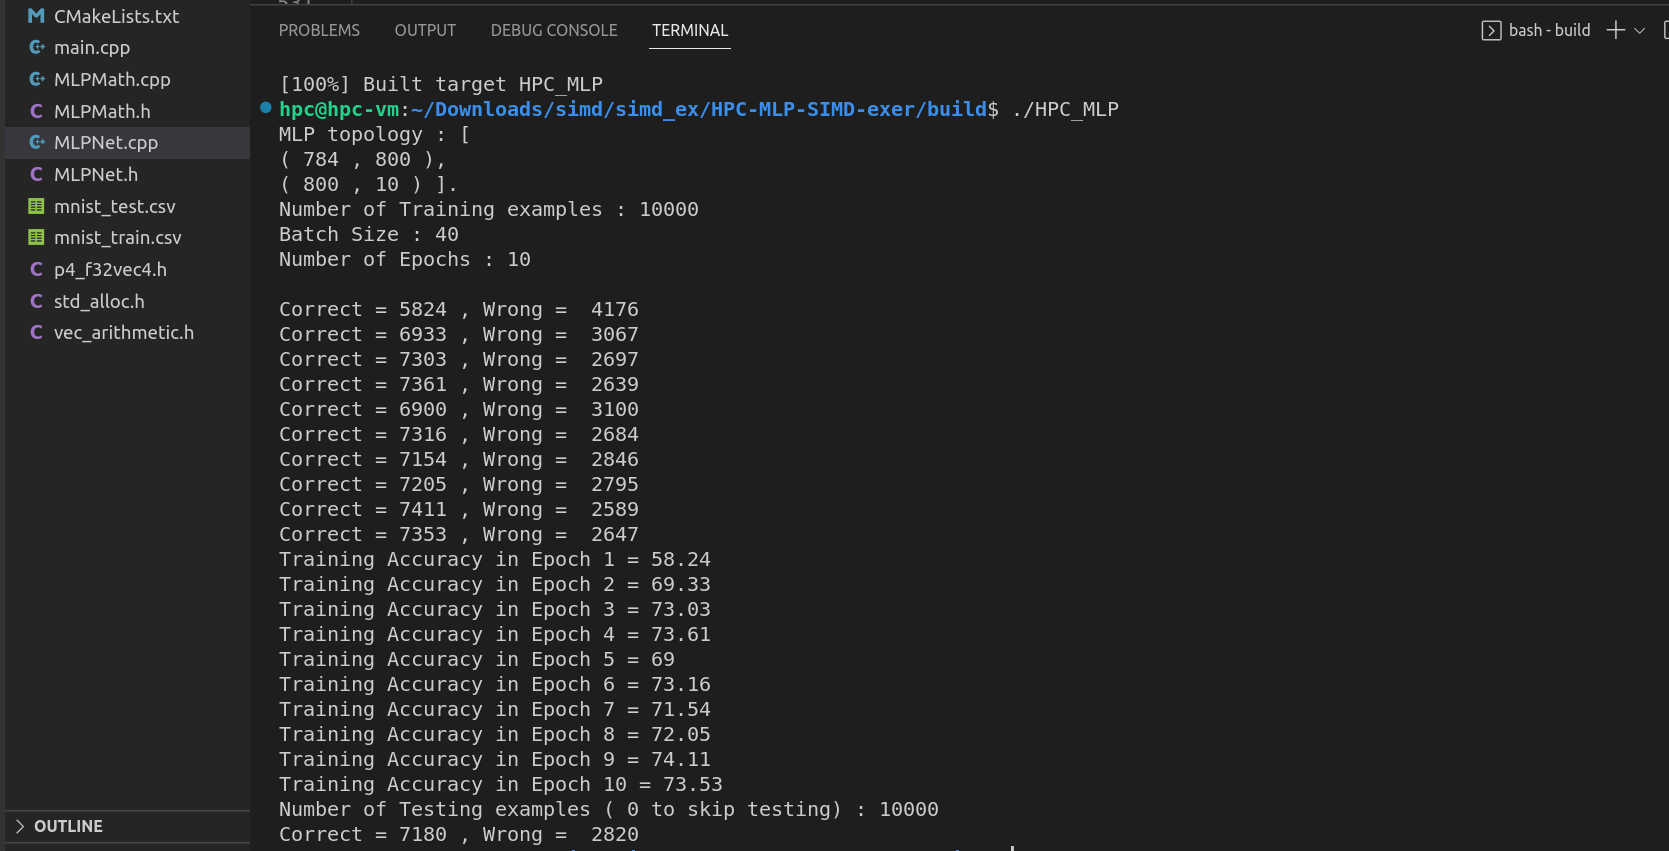
\includegraphics[scale=0.5]{ex_03_output.png} 
    \caption{Output}
    \label{fig:example}
  \end{figure}

\paragraph{}
The peak training accuracy of 74.11 in epoch 9 and a testing accuracy of  71.80 is recorded when we run the program on the data. 


\section{Matrix}
In this task we need to speed up Matrix calculations using SIMD.
As displayed below, we want to go from matrix a to matrix c.

\[
a = \begin{bmatrix}
a_0 & a_1 & a_2 \\
a_3 & a_4 & a_5 \\
a_6 & a_7 & a_8
\end{bmatrix}
\]

\[
c = \begin{bmatrix}
\sqrt{a_0} & \sqrt{a_1} & \sqrt{a_2} \\
\sqrt{a_3} & \sqrt{a_4} & \sqrt{a_5} \\
\sqrt{a_6} & \sqrt{a_7} & \sqrt{a_8}
\end{bmatrix}
\]
\newpage

\noindent First of all we need to change the input \& output matrices (output for scalar computation stays the same).
We do this by changing the memory alignment of the values of the matrices.
This is a requirement for SIMD-ized operations.
\begin{lstlisting}[caption=Matrix.cpp]
float a[N][N] __attribute__((aligned(16)));      // input array
float c[N][N]; // output array for scalar computations
float c_simd[N][N] __attribute__((aligned(16))); // output array for SIMD computations
\end{lstlisting}

\noindent The loops for the computation part remain mostly unchanged to the scalar version.
The inner loop runs N-times but our loop variable increases by 4, because each vector has 4 elements and those can the calculated in parallel.
We loop for $NIter - 1$ times, to neglect memory reading time.
Subsequently we loop over matrix a to transform it into matrix c (NxN for rows and columns).
The distinct section ranges from line 5 to line 7. We define two new vectors, called aVec and cVec, which suppose to be the vector counter parts to the scalar versions of matrix a and matrix c.
At the beginning those were initialized with float values, so we use the reinterpret\_cast command to allow treating
a variables memory representation as another type. In this case we substitute float for fvec.
Finally we just plug those values into the template function to calculate the root (Line 7).

\begin{lstlisting}[caption=Matrix.cpp]
TStopwatch timerSIMD;
for( int ii = 0; ii < NIter; ii++ )
    for( int i = 0; i < N; i++ ) {
        for( int j = 0; j < N; j++ ) {
            fvec &aVec = reinterpret_cast<fvec&>(a[i][j]);
            fvec &cVec = reinterpret_cast<fvec&>(c_simd[i][j]);
            cVec = f(aVec);
        }
    }
timerSIMD.Stop();
\end{lstlisting}

\noindent We can compute 4 values in parallel and therefore can expect a speed-up factor of 4. Due to running environment deviation, the speed-up factor varies.
\begin{figure}[H]
    \centering
    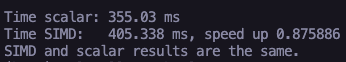
\includegraphics[scale=0.5]{matrix-output.png} 
    \caption{Output}
    \label{fig:example}
  \end{figure}
\section{Quadratic Equation}
\subsection{Quadratic Equation - Copying of data, SIMD}
In this task we first need to create a copy of the
data into a \_\_m128 datatype. For this, we use the
function \_mm\_set\_ps. This function takes 4 float values
and concating them in mirrored order.
Now we need to calculate the root - here we use
the predefined functions (\_mm\_div\_ps, ...).
\subsection{Quadratic Equation - Casting, SIMD}
Here there is not much different to the exercise above.
We need to cast the data into a \_\_m128 datatype with the
reinterpret\_cast function.
Then we can again use the predefined functions to calculate
the root like before.
\subsection{Quadratic Equation - Copying of data, fvec}
We first copy the data with defining the fvecs
(takes 4 arguments - 32 bit).
Then we calculate as usual.
\subsection{Quadratic Equation - Casting, fvec}
In this exercise we need to cast the data
like in one of the previous exercises. We
did this with the reinterpret\_cast function.
Then we can calculate the root as usual.



\subsection{Quadratic Equation - Output}
Time scalar: 75.4349 ms\\
Time SIMD1:    34.869 ms, speed up 2.16338\\
Time SIMD2:    34.0381 ms, speed up 2.21619\\
Time SIMD3:    35.1319 ms, speed up 2.14719\\
Time SIMD4:    35.0568 ms, speed up 2.15179\\
SIMD1 and scalar results are the same.\\
SIMD2 and scalar results are the same.\\
SIMD3 and scalar results are the same.\\
SIMD4 and scalar results are the same.\\

\subsection{Quadratic Equation - Time}
The data computed is for all the options the
same - 10000 vectors. Theoretically the times
should be quartered, but it differs a bit.



\section{CheckSum}
To get the checksum, we need to XOR over all the bytes of the array. If we want to use 
the SIMD-ized version, we need to XOR over all in parallel.
To do this, we first need to map the array to fvecs - reinterpret\_cast. This datatype is needed 
for the XOR with SIMD.
Then we can use the template command to XOR over all the bytes in parallel.
The result is a fvec, which we need to map back to a char. This is done by using the
reinterpret\_cast command again. After we iterated over the resulting char-array
and XORed over all the bytes, we get the checksum. Now we can stop the timer.
\\\\
If we want to parallelize without SIMD,
we map the the array to integers (4:1). This array
is XORED and we have a vector with 4 checksums.
To get the final checksum, we need to XOR over all the 4 checksums.
And again, we stop the time.
\subsection{CheckSum-Result}
The speedup we've got with the Time SIMD is only 8.32 - in
theory it should be close to 16 (because of the parallel 
computations), but in reality there is a bit of difference.
The speed up of the Scalar Integer is about 4 (3.91) and 
pretty much what we expected - 4 bytes per integer.
\subsection{CheckSum-Output}
Time scalar: 112.757 ms\\
Time INT: 28.821 ms, speed up 3.91232\\
Time SIMD: 13.551 ms, speed up 8.32094\\
Results are the same.

\section{Appendix}
\subsection{ReLU}\label{subsec:ReLU}
\begin{center}
    \begin{tikzpicture}
    \begin{axis}[
        xlabel={$x$},
        ylabel={$y$},
        axis lines=middle,
        xmin=-5, xmax=5,
        ymin=-0.5, ymax=5,
        xtick={-5,-4,-3,-2,-1,0,1,2,3,4,5},
        ytick={0,1,2,3,4,5},
        yticklabels={0,1,2,3,4,5},
        xticklabels={-5,-4,-3,-2,-1,0,1,2,3,4,5},
        samples=100,
        domain=-5:5,
        smooth,
        thick
    ]
    \addplot+[mark=none] {max(0,x)};
    \end{axis}
    \end{tikzpicture}
    \end{center}
    \[
    \text{ReLU}(x) =
    \begin{cases}
    x, & \text{if } x \geq 0 \\
    0, & \text{otherwise}
    \end{cases}
    \]


\end{document}
